\section{\evopolicygym{}: A Framework for Autonomous Policy Evolution}
\label{sec:framework}


\begin{figure*}[t]
    \centering
    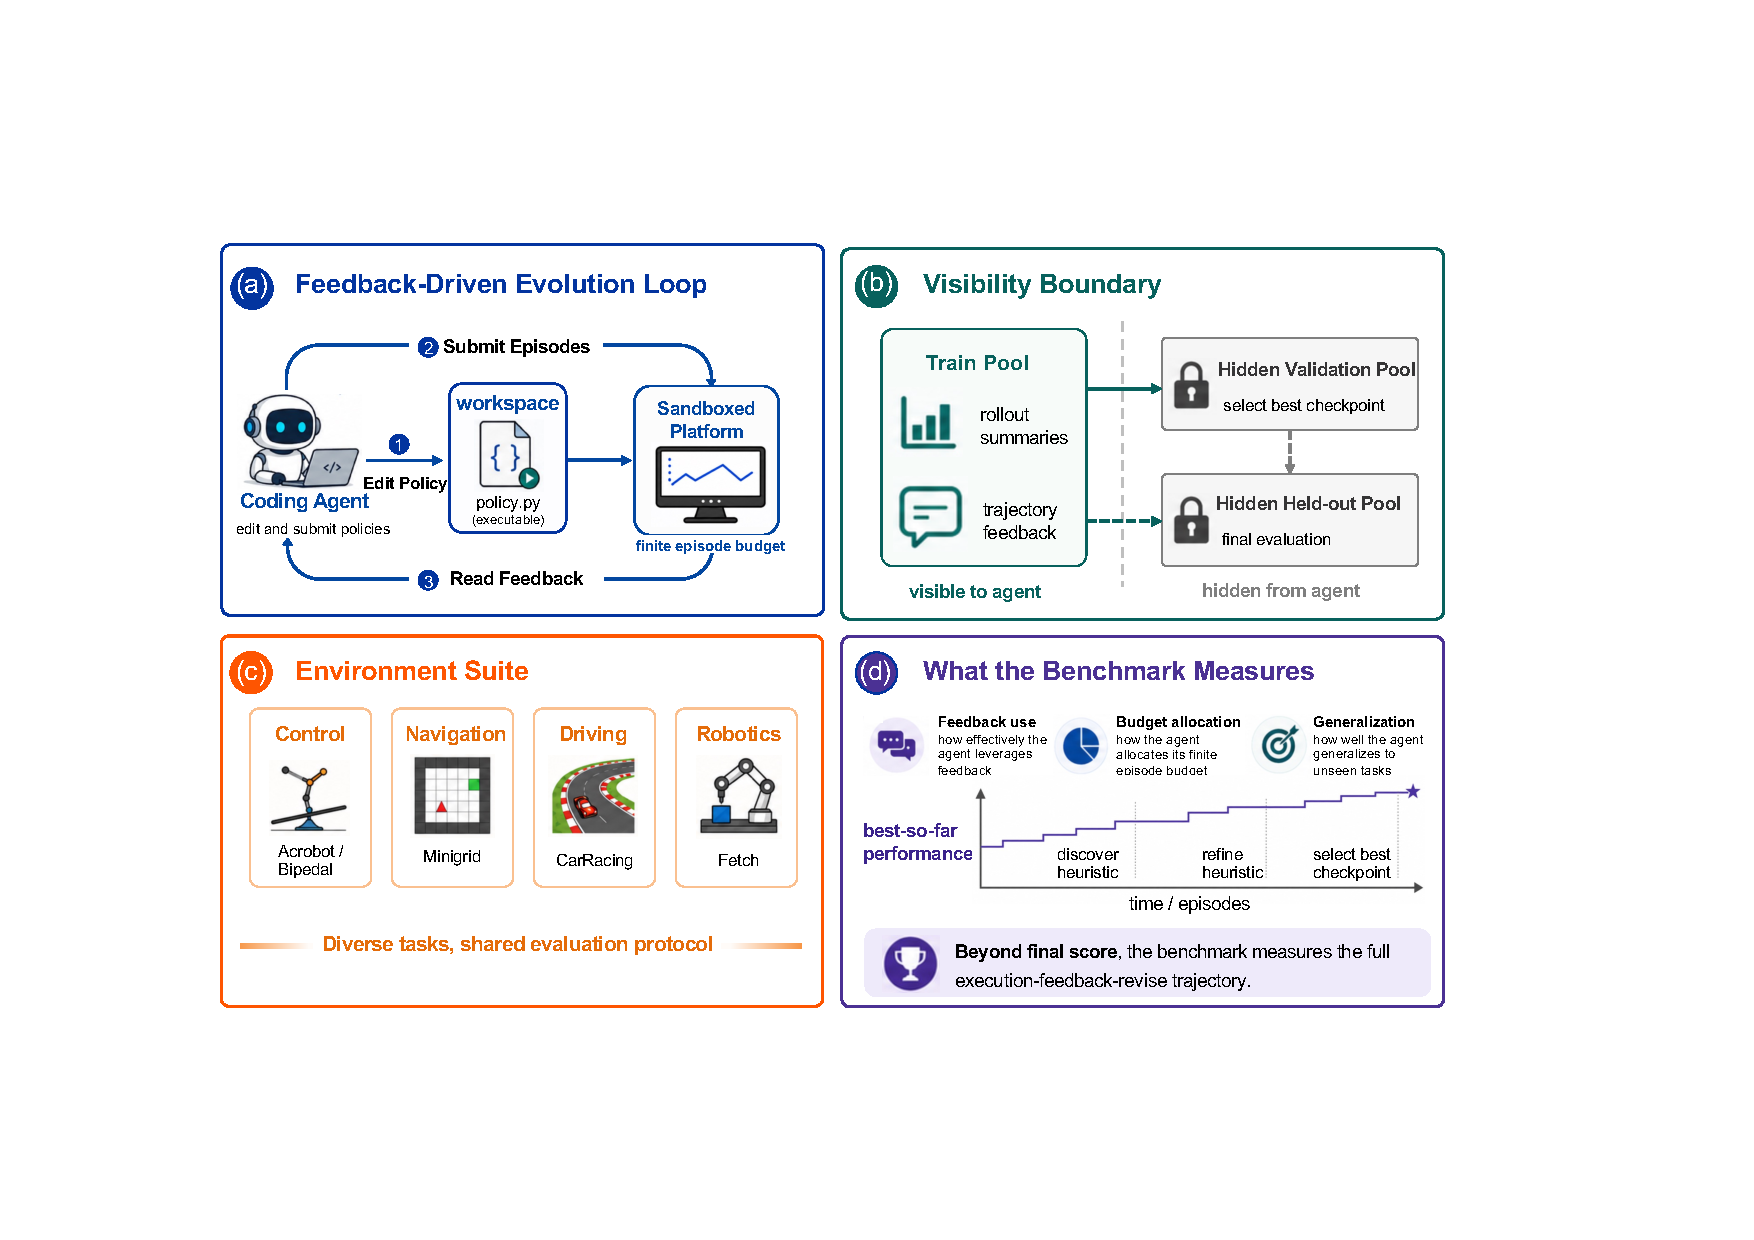
\includegraphics[width=0.98\textwidth]{figs/mainfig.pdf}
    \caption{\small
    \textbf{EvoPolicyGym framework.} (a) \textbf{Interaction loop}: agents edit policies, submit episodic rollouts under a finite budget, and receive platform-mediated feedback. 
    (b) \textbf{Visibility boundary}: training feedback is visible, while validation-based checkpoint selection and held-out evaluation are hidden.
    (c) \textbf{Environment suite}: a unified interface spanning control, navigation, driving, and robotics tasks under a shared evaluation protocol. 
    (d) \textbf{Measured aspects}: feedback utilization, budget efficiency, and policy improvement dynamics, captured via the evolution of best-so-far performance over time.
    }
    % \caption{
    %     Main \evopolicygym{} online optimization protocol.
    %     The agent sees the workspace-facing interfaces and self-evolves by
    %     editing \texttt{system/}, submitting train episodes, and reading
    %     \texttt{feedback/}. Server-owned finalization remains hidden:
    %     validation selects the best strategy and heldout evaluation writes the
    %     final score to \texttt{run.json}.
    % }
    \label{fig:online-submit-protocol}
\end{figure*}


\evopolicygym{} frames autonomous policy evolution as an agent-driven
optimization loop for executable decision policies. In each run, a coding agent
maintains a persistent policy workspace, submits candidate revisions for visible
train episodes, receives server-generated rollout summaries and trajectories,
and revises the policy under a fixed episode budget. 
The primary evaluation unit is a complete budget-constrained run, scored by the held-out return of its best validation checkpoint. The associated trajectory provides diagnostic evidence about how that outcome was reached.
Figure~\ref{fig:online-submit-protocol} summarizes the visible workspace
interfaces, the submission loop, and server-owned finalization.
%\runzhe{this phrase conflicts with the scoring rule, which uses the held-out return of one validation-selected checkpoint. from my understanding, trajectories support diagnosis rather than leaderboard scoring}
%\runzhe{suggested edit: The primary evaluation unit is a complete budget-constrained run, scored by the held-out return of its best validation checkpoint. The associated trajectory provides diagnostic evidence about how that outcome was reached.}

\subsection{Environment, Policy, and Interaction}
\label{sec:task-objects}

Before specifying the benchmark protocol, we define the three objects that make
a policy-evolution task executable: an environment, a policy system, and an
episode. The definitions use the common \texttt{reset}/\texttt{step}
environment interface \citep{gymnasium}, but are stated in benchmark-facing
terms because 
%\evopolicygym{} evaluates coding agents \runzhe{these days, everyone is calling it a ``coding agent'', right?} that optimize
executable decision policies.

\paragraph{Environment.}
An \emph{environment} is an interactive task in which a policy acts. It exposes
observations, accepts actions, and returns rewards that measure task progress.
A reset initializes an episode; each later \texttt{step(action)} advances the
environment and returns the next observation, reward, and termination status.
Observations may be pixels, vectors, dictionaries, or symbolic grids, and
actions may be discrete choices or continuous controls.

\paragraph{Policy.}
A \emph{policy} is the decision rule that chooses actions using observations
and any information it has retained from earlier interaction. We write this
memory as an internal state $h_t$. A deterministic policy maps
$(o_t,h_t)$ to an action and updated internal state,
$(a_t,h_{t+1})=\mu(o_t,h_t)$. A stochastic policy analogously samples
$(a_t,h_{t+1}) \sim \pi(\cdot \mid o_t,h_t)$. In \evopolicygym{}, the
stateful mapping is implemented by the executable Python artifact that the coding agent writes and the judge later runs. Its minimal judge-facing interface is an object with \texttt{reset} at the start of an episode and \texttt{act(obs)} at each step; the internal state is maintained behind this interface. The artifact may also include helper modules, constants, planners, controllers, diagnostics, or learned parameters. We call this whole executable bundle the \emph{policy system}.
%\runzhe{concerns regarding the policy notation... too restrictive here. a stateful policy is not generally a function of $o_t$ alone because our experimental environment explicitly permits memory. formally, define an internal state $h_t$ here, so that we can derive $(a_t,h_{t+1})=\mu(o_t,h_t)$, with the stochastic analogue if needed. then, reserve ``policy system'' for the executable bundle that implements this stateful mapping}

\begin{figure}[t]
\centering
\begin{minipage}[t]{0.485\linewidth}
\textbf{Gymnasium-style env (server-owned)}
\begin{tcblisting}{
  enhanced,
  listing only,
  equal height group=env-policy-api,
  width=\linewidth,
  colback=cardbg,
  colframe=accent,
  boxrule=0.35pt,
  arc=2pt,
  left=6pt,
  right=6pt,
  top=4pt,
  bottom=4pt,
  boxsep=0pt,
  listing options={
    language=Python,
    basicstyle=\ttfamily\scriptsize,
    keywordstyle=\color{accent}\bfseries,
    commentstyle=\color{black!55},
    stringstyle=\color{black!70},
    emph={Environment,reset,step},
    emphstyle=\color{accent}\bfseries,
    columns=fullflexible,
    keepspaces=true,
    showstringspaces=false,
    breaklines=true,
    breakatwhitespace=true
  }
}
class Environment:
    observation_space = ...
    action_space = ...

    def reset(self, *, seed=None,
              options=None): ...
    # -> obs, info

    def step(self, action): ...
    # -> obs, reward, terminated,
    #    truncated, info
\end{tcblisting}
\end{minipage}
\hfill
\begin{minipage}[t]{0.485\linewidth}
\textbf{Policy-system entry point}
\begin{tcblisting}{
  enhanced,
  listing only,
  equal height group=env-policy-api,
  width=\linewidth,
  colback=cardbg,
  colframe=accent,
  boxrule=0.35pt,
  arc=2pt,
  left=6pt,
  right=6pt,
  top=4pt,
  bottom=4pt,
  boxsep=0pt,
  listing options={
    language=Python,
    basicstyle=\ttfamily\scriptsize,
    keywordstyle=\color{accent}\bfseries,
    commentstyle=\color{black!55},
    stringstyle=\color{black!70},
    emph={Policy,__init__,reset,act},
    emphstyle=\color{accent}\bfseries,
    columns=fullflexible,
    keepspaces=true,
    showstringspaces=false,
    breaklines=true,
    breakatwhitespace=true
  }
}
class Policy:
    def __init__(self, obs_space,
                 action_space, env_meta): ...

    def reset(self, episode_index): ...
    # -> None

    def act(self, obs): ...
    # -> action


    
\end{tcblisting}
\end{minipage}
\caption{Minimal runtime boundary for one \evopolicygym{} episode. The server
owns the Gymnasium-style environment, which maps actions to observations and
rewards. The submitted policy system maps observations to actions through this
entry point, but may internally contain helper modules, planners, memory,
diagnostics, learned parameters, or other decision logic.}
\label{fig:environment-policy-api}
\end{figure}

\paragraph{Episode.}
An \emph{episode} is one complete policy--environment interaction. It begins
with an environment reset and ends at termination or truncation. At time $t$,
the policy receives observation $o_t$, returns action $a_t$, and the environment
produces reward $r_t$ and the next observation. The episode is the basic
evaluation unit in \evopolicygym{}; its \emph{return} is the cumulative reward
collected during the interaction, and higher return is better in our benchmark.

\subsection{Autonomous Policy Evolution Protocol}
\label{sec:ape}


\evopolicygym{} evaluates the ability of a coding agent to optimize an
executable policy system from environment feedback. A run begins with one
environment, an initial policy workspace, and a fixed episode budget. Over the
run, the agent inspects the workspace, reads feedback from previous
submissions, edits code, and decides when to submit the current artifact and
how much of the remaining episode budget to spend on evaluation.

At observed revision $i$, let $W_i$ denote the workspace state visible to the
agent, $F_i$ the server-written feedback from prior submissions, and $B_i$ the
remaining episode budget. The current executable policy system is induced by
the workspace, written $P_i=\Phi(W_i)$. We denote the coding agent by
$\pi_\theta$, a language model together with its tool-using harness. The agent
observes $(W_i,F_i,B_i)$, carries history $\mathcal{H}_i$, and writes patches
to the workspace.
Figure~\ref{fig:online-submit-protocol} organizes the same loop around the
\emph{Agent}, \emph{Workspace}, and \emph{Server}.

The run induces a sequence of observed-state transitions:
\[
\pi_\theta(W_i, F_i, B_i, \mathcal{H}_i)
\rightarrow (u_i,s_i,\mathcal{H}_{i+1}),\qquad
s_i\in\{\bot\}\cup\mathcal{C}(B_i),
\]
\[
W_{i+1}=\mathrm{apply}(W_i,u_i),\qquad
P_{i+1}=\Phi(W_{i+1}),
\]
\[
(\Delta F_i,c_i)=S(B_i,P_{i+1},s_i),\qquad
B_{i+1}=B_i-c_i,\qquad
F_{i+1}=F_i\cup\Delta F_i.
\]
Here $\mathcal{H}_i$ is the agent's accumulated conversational and tool-use
history, $u_i$ is a workspace patch, and $s_i$ is a server-facing submit
command. The null command $s_i=\bot$ means that no train evaluation is requested
at this revision; otherwise $s_i\in\mathcal{C}(B_i)$ specifies a valid train
submit under the remaining episode budget. A patch may tune constants, add
helper modules, introduce memory, replace a controller, add diagnostics, or
restructure the policy system induced by the workspace. The server operator $S$
returns the new feedback $\Delta F_i$ and charged episode count $c_i$. It sets
$c_i=0$ and returns no new feedback when $s_i=\bot$ or no evaluation is
accepted; otherwise it snapshots the selected revision, charges the accepted
train episodes, and returns feedback for later patches. Submit commands do not
themselves modify $W_i$ or $P_i$. After the run ends, the server
automatically performs hidden validation selection and held-out evaluation.
Final scores therefore compare each agent's optimization outcome under the same episode budget.


\FloatBarrier
\subsection{Feedback and Evaluation Boundary}
\label{sec:feedback-signals}

The agent obtains environment evidence only through submitted train episodes.
For each accepted submit, the server evaluates a snapshot of the current policy
system, charges one budget unit per requested episode, and writes the
observable feedback signal $F_i$. Feedback includes structured summaries,
episode returns and statuses, trajectory records, diagnostic streams, error
reports, and optional environment-specific artifacts such as frames or videos.
These signals guide the next update $u_i$ to $P_i$.

A fixed visibility boundary separates online feedback from final evaluation.
Train episodes provide in-loop rollout evidence; validation and held-out
evidence remain hidden until the optimization loop ends.
%validation score -> post-hoc diagnostics in Section 4.3
%\runzhe{Also call the score evolution curves in Section~\ref{sec:score-evolution}: post-hoc diagnostics wherever they first appear, so readers cannot mistake hidden validation for an optimization signal.} 
The server then
selects a checkpoint by hidden validation and reports its hidden held-out
performance.
Appendix~\ref{app:evaluation-and-scoring} gives the detailed visibility table,
scoring rule, and audit traces.

\subsection{Environment Abstraction and Extensibility}
\label{sec:gym-compatible-envs}

The environment layer is separated from the agent protocol. Any
Gymnasium-compatible episodic environment with a \texttt{reset}/\texttt{step}
interface can be wrapped by an adapter that implements reset, step, and
reproducible episode initialization. The adapter converts observations and
actions into compact schemas, loads reproducible train/validation/held-out
initialization splits, and keeps hidden split metadata outside the agent
workspace.


This design keeps interaction, visibility, budget, and artifact semantics fixed
as environment coverage grows. We distinguish adapter-level support from full
experimental validation. At the adapter level, the current implementation
includes Gymnasium-style wrappers and interface tests for Classic Control, Toy
Text, Box2D, MuJoCo, Atari/ALE, MiniGrid, MiniWorld, HighwayEnv,
Gymnasium-Robotics, MO-Gymnasium, BrowserGym, MiniWoB++, and MetaWorld. These
tests check that tasks can be reset, stepped, initialized from reproducible
splits, and exposed through the common observation/action schema. At the
experimental level, this paper validates the full protocol on the calibrated
Core16 subset, which uses 16 tasks spanning Gym/Box2D, MuJoCo, MiniGrid, and
robotics/driving environments. The broader adapter surface serves as a task
reservoir from which future experiments can select additional calibrated
subsets.
%\runzhe{Distinguish implemented and validated support from packages merely available in the environment. Or weaken the claim to: ``The adapter design is compatible with these Gymnasium-style families; the present study validates the protocol on the xxxxx subset.''}
